%%
%% ****** ljmsamp.tex 13.06.2018 ******
%%
\documentclass[
11pt,%
tightenlines,%
twoside,%
onecolumn,%
nofloats,%
nobibnotes,%
nofootinbib,%
superscriptaddress,%
noshowpacs,%
centertags]%
{revtex4-2}
\usepackage{ljm}
\begin{document}

\titlerunning{Sufficient Sample Size Estimation: Posterior Distributions Proximity} % for running heads
\authorrunning{Nikita Kiselev, Andrey Grabovoy} % for running heads
%\authorrunning{First-Author, Second-Author} % for running heads

\title{Sufficient Sample Size Determination:\\ Posterior Distributions Proximity}
% Splitting into lines is performed by the command \\
% The title is written in accordance with the rules of capitalization.

\author{\firstname{N.~S.}~\surname{Kiselev}}
\email[E-mail: ]{kiselev.ns@phystech.edu}
\affiliation{Moscow Institute of Physics and Technology, 9 Institutskiy per., Dolgoprudny, Moscow Region, 141701, Russian Federation}

\author{\firstname{A.\,V.}~\surname{Grabovoy}}
\email[E-mail: ]{grabovoy.av@phystech.edu}
\affiliation{Moscow Institute of Physics and Technology, 9 Institutskiy per., Dolgoprudny, Moscow Region, 141701, Russian Federation}
%\noaffiliation % If the author does not specify a place of work.

%\firstcollaboration{(Submitted by A.~A.~Editor-name)} % Add if you know submitter.
%\lastcollaboration{ }

%\received{June 13, 2018} % The date of receipt to the editor, i.e. December 06, 2017


\begin{abstract} % You shouldn't use formulas and citations in the abstract.
    The paper investigates the problem of estimating a sufficient sample size. The issue of determining a sufficient sample size without specifying a statistical hypothesis about the distribution of model parameters is considered. Two approaches to determining a sufficient sample size based on the proximity of posterior distributions of model parameters on similar subsets are suggested. The correctness of the presented approaches is proven in the model with normal posterior distribution. A theorem about moments of the limit posterior distribution of parameters in a linear regression model is proven. A computational experiment is conducted to analyze the properties of the proposed methods.
\end{abstract}

%\subclass{12345, 54321} % Enter 2010 Mathematics Subject Classification.

\keywords{Sufficient sample size, Posterior distributions proximity, Bayesian inference, Linear regression} % Include keywords separeted by comma.

\maketitle

% Text of article starts here.

% ====================
\section{Introduction}
% ====================

The task of supervised machine learning involves selecting a predictive model from a parametric family. This choice is usually based on certain statistical hypotheses, such as maximizing a quality functional. A model that satisfies these statistical hypotheses is called an \textit{adequate} model \cite{bies2006genetic, cawley2010over, raschka2018model}.

When planning a computational experiment, it is necessary to estimate the minimum sample size~--- the number of objects required to build an adequate model. The sample size required to build an adequate predictive model is called \textit{sufficient} \cite{byrd2012sample, figueroa2012predicting, balki2019sample}. 

This work addresses the issue of determining the sufficient sample size. There are numerous studies dedicated to this topic, with approaches classified into statistical, Bayesian, and heuristic methods.

Some of the early researches on this topic \cite{Adcock1988, Joseph1995} formulate a specific statistical criterion, where the sample size estimation method associated with this criterion guarantees achieving a fixed statistical power with a Type I error not exceeding a specified value. Statistical methods include the Lagrange multipliers test \cite{self1988power}, the Likelihood ratio test \cite{shieh2000power}, the Wald statistic \cite{shieh2005power}. Statistical methods have certain limitations associated with their practical application. They allow for estimating the sample size based on assumptions about the data distribution and information about the agreement of observed values with the assumptions of the null hypothesis.

The Bayesian approach also has a place in this problem. In the work \cite{Lindley1997} the sufficient sample size is determined based on maximizing the expected utility function. This may explicitly include parameter distribution functions and penalties for increasing the sample size. This work also considers alternative approaches based on constraining a certain quality criterion for estimating model parameters. Among these criteria, the Average Posterior Variance Criterion (APVC), Average Coverage Criterion (ACC), Average Length Criterion (ALC), and Effective Sample Size Criterion (ESC) stand out. These criteria have been further developed in other works, for example, \cite{PhamGia1997} and \cite{Gelfand2002}. Over time, the authors of \cite{Cao2009} conducted a theoretical and practical comparison of methods from \cite{Adcock1988, Joseph1995, Lindley1997}.

Authors like \cite{Brutti2014}, as well as \cite{Pezeshk2008}, discuss the differences between Bayesian and frequentist approaches in determining sample size. They also propose robust methods for the Bayesian approach and provide illustrative examples for some probabilistic models.

In the paper \cite{Grabovoy2022}, various methods for estimating sample size in generalized linear models are considered, including statistical, heuristic, and Bayesian methods. Methods such as Lagrange Multiplier Test, Likelihood Ratio Test, Wald Test, Cross-Validation, Bootstrap, Kullback-Leibler Criterion, Average Posterior Variance Criterion, Average Coverage Criterion, Average Length Criterion, and Utility Maximization are analyzed. The authors point out the potential development of combining Bayesian and statistical approaches to estimate sample size for insufficient available sample sizes.

In \cite{MOTRENKO2014743} a method for determining sample size in logistic regression is discussed, using cross-validation and Kullback-Leibler divergence between posterior distributions of model parameters on similar subsamples. Similar subsamples are those that can be obtained from each other by adding, removing, or replacing one object.

In this paper, two approaches based on the distance between the posterior distributions are presented. It is proposed to consider two similar subsamples. The posterior distributions of the model parameters over these subsamples turn out to be close if the sample size is sufficient. It is proposed to use the Kullback-Leibler divergence \cite{MOTRENKO2014743} as a measure of the proximity of distributions, as well as the s-score model comparison function \cite{Aduenko2017}. The novelty of this work lies in proving the correctness of the proposed methods. Correctness is proved in a probabilistic model with a normal posterior distribution of parameters. For the linear regression model, the theorem on the moments of the limit posterior distribution of parameters is proved.

% =========================
\section{Problem statement}
% =========================

An object is defined as a pair $(\mathbf{x}, y)$, where $\mathbf{x} \in \mathbb{X} \subseteq \mathbb{R}^n$ is the feature vector, and $y \in \mathbb{Y}$ is the target variable. In regression problems $\mathbb{Y} = \mathbb{R}$, and in $K$-class classification problems $\mathbb{Y} = \{1, \ldots, K\}$.

The feature-object matrix for a sample $\mathfrak{D}_m = \left\{ (\mathbf{x}_i, y_i) \right\}, i \in \mathcal{I} = \{ 1, \ldots, m \}$ of size $m$ is called the matrix $\mathbf{X}_m = \left[ \mathbf{x}_1, \ldots, \mathbf{x}_m \right]^{\top} \in \mathbb{R}^{m \times n}$.

The target variable vector for a sample $\mathfrak{D}_m = \left\{ (\mathbf{x}_i, y_i) \right\}, i \in \mathcal{I} = \{ 1, \ldots, m \}$ of size $m$ is denoted by $\mathbf{y}_m = \left[ y_1, \ldots, y_m \right]^{\top} \in \mathbb{Y}^m$.

A model is a parametric family of functions $f$, mapping the Cartesian product of the set of feature vector values $\mathbb{X}$ and the set of parameter values $\mathbb{W}$ to the set of target variable values $\mathbb{Y}$: 
\[ f: \mathbb{X} \times \mathbb{W} \to \mathbb{Y}. \]

A probabilistic model is a joint distribution
\[ p(y, \mathbf{w} | \mathbf{x}) = p(y | \mathbf{x}, \mathbf{w}) p(\mathbf{w}): \mathbb{Y} \times \mathbb{W} \times \mathbb{X} \to \mathbb{R}^+, \]
where $\mathbf{w} \in \mathbb{W}$ is the set of model parameters, $p(y | \mathbf{x}, \mathbf{w})$ specifies the likelihood of an object, and $p(\mathbf{w})$ represents the prior distribution of parameters.

The likelihood function of a sample $\mathfrak{D}_m = \left\{ (\mathbf{x}_i, y_i) \right\}, i \in \mathcal{I} = \{ 1, \ldots, m \}$ of size $m$, where $\mathbf{x}_1, \ldots, \mathbf{x}_m$ are i.i.d. together, is defined as 
\[ L(\mathfrak{D}_m, \mathbf{w}) = p(\mathbf{y}_m | \mathbf{X}_m, \mathbf{w}) = \prod_{i=1}^{m} p(y_i | \mathbf{x}_i, \mathbf{w}). \]
Its logarithm
\[ l(\mathfrak{D}_m, \mathbf{w}) = \sum\limits_{i=1}^{m} \log p(y_i | \mathbf{x}_i, \mathbf{w}) \]
is called the logarithmic likelihood function. Unless stated otherwise, we consider samples to be i.i.d.

The maximum likelihood estimate of a set of parameters $\mathbf{w} \in \mathbb{W}$ based on the subsample $\mathfrak{D}_k$ of size $k$ is given by 
\[ \hat{\mathbf{w}}_{k} = \arg\max_{\mathbf{w} \in \mathbb{W}} L(\mathfrak{D}_k, \mathbf{w}). \]

The task is to determine the sufficient sample size $m^*$. Let a criterion $T$ be given. E.g. it can be constructed based on heuristics regarding the behaviour of model parameters.
\begin{definition}
    The sample size $m^*$ is called \textbf{sufficient} according to the criterion $T$, if $T$ holds for all $k \geqslant m^*$.
\end{definition}

% ============================================================================
\section{Proposed sample size determination methods}\label{sec2}
% ============================================================================

In \citep{MOTRENKO2014743}, it is suggested to use the Kullback-Leibler divergence to estimate a sufficient sample size in a binary classification problem. The idea is based on the fact that if two subsamples differ from each other by one object, then the posterior distributions obtained from them should be close. This proximity is determined by the Kullback-Leibler divergence. 

In this paper, the question of the correctness of this approach is considered. The method is studied in an arbitrary probabilistic model. As a measure of proximity, it is proposed to use not only the Kullback-Leibler divergence, but also the s-score similarity function from \citep{Aduenko2017}.

Consider two subsamples $\mathfrak{D}^1\subseteq\mathfrak{D}_m$ and $\mathfrak{D}^2\subseteq\mathfrak{D}_m$. Let $\mathcal{I}_1 \subseteq \mathcal{I} = \{1, \ldots, m\}$ and $\mathcal{I}_2 \subseteq \mathcal{I} =\{1, \ldots,m\}$~--- corresponding to them subsets of indexes.

\begin{definition}
    Subsamples $\mathfrak{D}^1$ and $\mathfrak{D}^2$ are called \textbf{similar} if $\mathcal{I}_2$ can be obtained from $\mathcal{I}_1$ by deleting, replacing or adding one element, that is
    \[ \left| \mathcal{I}_1 \triangle \mathcal{I}_2 \right| = \left| \left( \mathcal{I}_1 \setminus \mathcal{I}_2 \right) \cup \left( \mathcal{I}_2 \setminus \mathcal{I}_1 \right) \right| = 1. \]
\end{definition}

Consider two similar subsamples $\mathfrak{D}_k = (\mathbf{X}_k,\mathbf{y}_k)$ and $\mathfrak{D}_{k+1} = (\mathbf{X}_{k+1}, \mathbf{y}_{k+1})$ of sizes $k$ and $k+1$, respectively. This means that the larger one is obtained by adding one element to the smaller one. Let's find the posterior distribution of the model parameters over these subsamples:
\[p_j(\mathbf{w}) = p(\mathbf{w} | \mathfrak{D}_j) = \dfrac{p(\mathfrak{D}_j | \mathbf{w}) p(\mathbf{w})}{p(\mathfrak{D}_j)} \propto p(\mathfrak{D}_j | \mathbf{w}) p(\mathbf{w}), \quad j = k, k+1. \]

\begin{definition}
    Let's fix some positive number $\varepsilon > 0$. The sample size $m^*$ is called \textbf{KL-sufficient} if for all $k\geqslant m^*$
    \[ KL(k) = D_{KL}(p_k \| p_{k+1}) = \int p_k(\mathbf{w}) \log{\dfrac{p_k(\mathbf{w})}{p_{k+1}(\mathbf{w})}} d\mathbf{w} \leqslant \varepsilon. \]
\end{definition}

For a pair of normal distributions, the Kullback-Leibler divergence has a fairly simple form. Assume that the posterior distribution is normal, that is, $p_k(\mathbf{w}) = \mathcal{N}\left(\mathbf{w}|\mathbf{m}_k, \mathbf{\Sigma}_k\right)$. Guided by the heuristic that the convergence of the moments of such a distribution should entail the proximity of posterior distributions on similar subsamples, the following statement can be formulated.

\begin{theorem}\label{theorem1}
    Let $\|\mathbf{m}_{k+1} - \mathbf{m}_k\|_2 \to 0$ and $\|\mathbf{\Sigma}_{k+1} - \mathbf{\Sigma}_k\|_{F}\to 0$ as $k\to \infty$. Then, in a model with a normal posterior distribution of parameters, the definition of a KL-sufficient sample size is correct. Namely, for any $\varepsilon > 0$, there is such a $m^*$ that for all $k\geqslant m^*$ $KL(k)\leqslant\varepsilon$ is satisfied.
\end{theorem}

In this paper, it is proposed to use the s-score similarity function from \citep{Aduenko2017} as a measure of proximity of distributions:
\[\text{s-score}(g_1, g_2) = \dfrac{\int_{\mathbf{w}} g_1(\mathbf{w}) g_2(\mathbf{w}) d\mathbf{w}}{\max_{\mathbf{b}} \int_{\mathbf{w}} g_1(\mathbf{w} - \mathbf{b}) g_2(\mathbf{w}) d\mathbf{w}}. \]

\begin{definition}
    Let's fix some positive number $\varepsilon > 0$. The sample size $m^*$ is called \textbf{S-sufficient} if for all $k\geqslant m^*$
    \[ S(k) = \text{s-score}(p_k, p_{k+1}) \geqslant 1-\varepsilon. \]
\end{definition}

As in the case of a KL-sufficient sample size, in a model with a normal posterior distribution, it is possible to write an expression for the criterion used. Thus, one more statement can be formulated.

\begin{theorem}\label{theorem2}
    Let $\|\mathbf{m}_{k+1} - \mathbf{m}_k\|_2\to 0$ as $k \to \infty$. Then, in a model with a normal posterior distribution of parameters, the definition of an S-sufficient sample size is correct. Namely, for any $\varepsilon > 0$, there is such a $m^*$ that for all $k\geqslant m^*$ $S(k)\geqslant 1-\varepsilon$ is satisfied.
\end{theorem}

Let the linear regression model have a normal prior distribution of parameters. By the conjugacy property of the prior distribution and likelihood, the posterior distribution is also normal. Thus, we come to one of the simplest examples of a model for which the theorems presented above are valid. In fact, simpler statements can be formulated for linear regression.

\begin{theorem}\label{theorem3}
    Let the sets of values of the features and the target variable be bounded, that is, $\exists M\in \mathbb{R}:$ $\|\mathbf{x}\|_2\leqslant M$ and $|y|\leqslant M$. If $\lambda_{\min}\left(\mathbf{X}^{\top}_k \mathbf{X}_k \right) = \omega(\sqrt{k})$ for $k\to \infty$, then in a linear regression model with a normal prior distribution of parameters $\|\mathbf{m}_{k+1} - \mathbf{m}_k\|_2\to 0$ and $\|\mathbf{\Sigma}_{k+1} - \mathbf{\Sigma}_k\|_{F}\to 0$ as $k\to \infty$.
\end{theorem}

% ============================================
\section{Computational experiment}\label{sec4}
% ============================================

An experiment is conducted to analyze the properties of the proposed methods for estimating a sufficient sample size. Synthetic data is generated from a linear regression model. The number of objects is 1000, the number of features is 20. One object is sequentially removed from the given sample until the number of objects in the subsample is equal to the number of features. This process is repeated $B=100$ times. 

Fig.~\ref{lambda} shows the asymptotic behavior of the minimum eigenvalue of the matrix $\mathbf{X}^\top \mathbf{X}$. We see that when the sample size tends to infinity, the minimum eigenvalue also tends to infinity. Meanwhile, as is necessary for the Theorem~\ref{theorem3}, the graph is higher than $\sqrt{k}$.

\begin{figure}[h!]
    \centering
    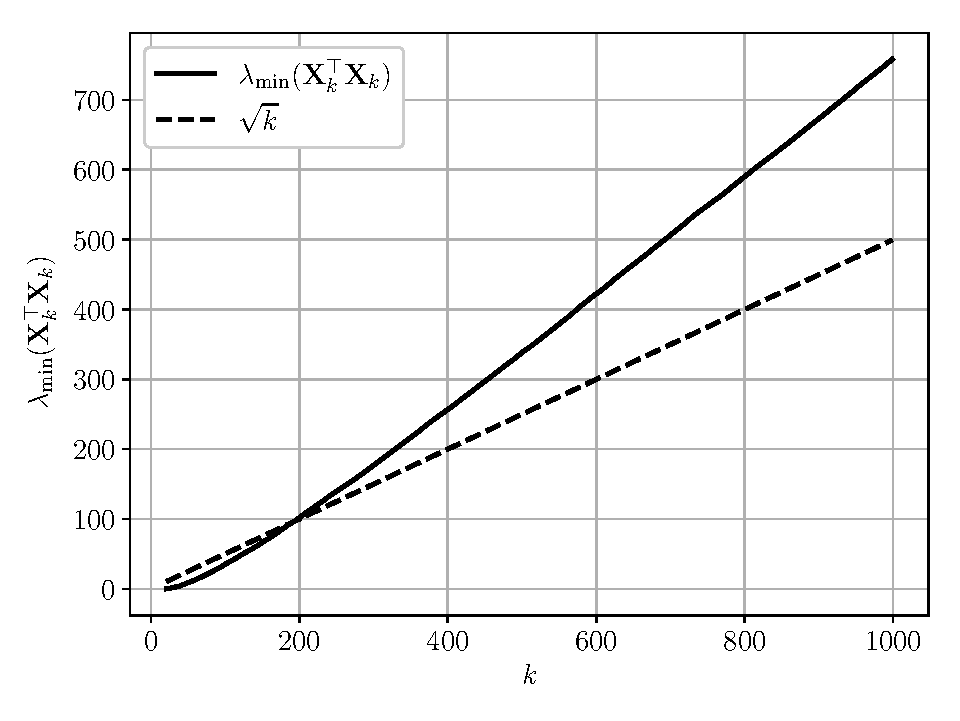
\includegraphics[width=0.5\textwidth]{../paper/figures/gray/eps/lambda}
    \caption{Asymptotics of the minimum eigenvalue}
    \label{lambda}
\end{figure}

For KL-sufficiency and S-sufficiency, $\varepsilon = 5 \cdot 10^{-2}$ was selected. The following is a Fig.~\ref{synthetic-regression-sufficient}, which shows the resulting dependencies of $KL(k)$ and $S(k)$. 

\begin{figure}[h!]
    \centering
    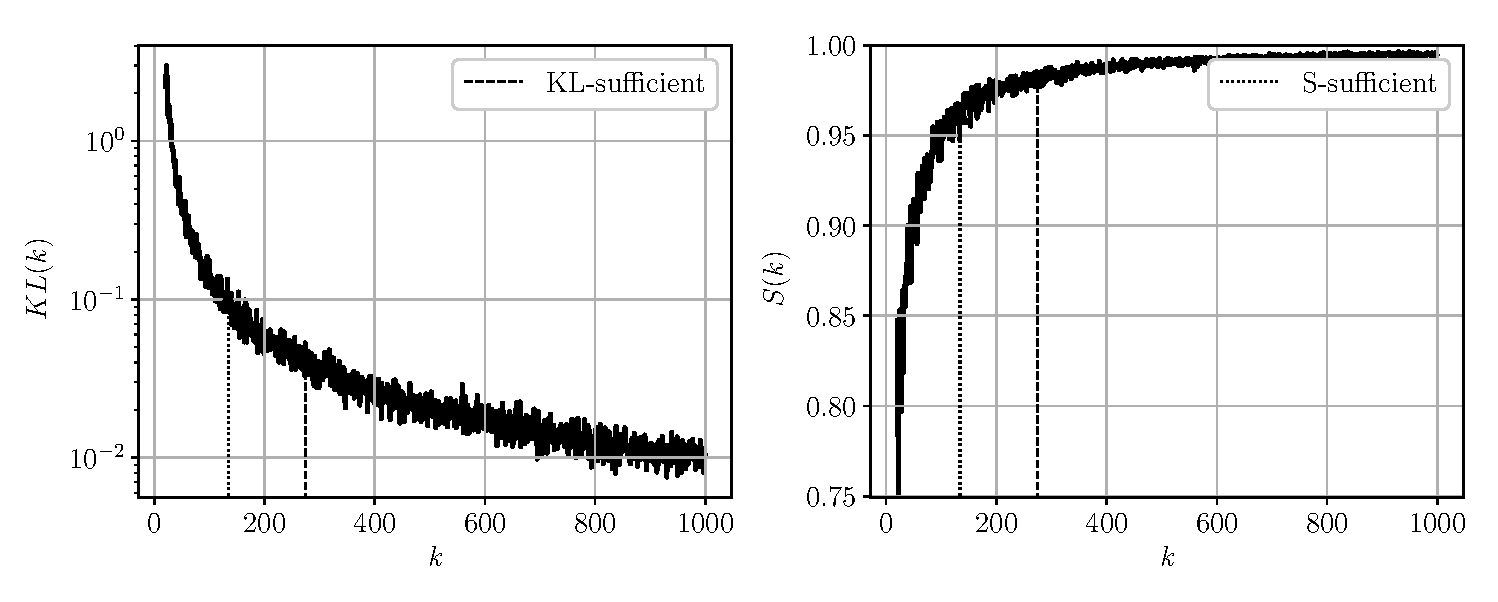
\includegraphics[width=0.9\textwidth]{../paper/figures/gray/eps/synthetic-regression-sufficient-KL-S}
    \caption{Synthetic sample (linear regression)}
    \label{synthetic-regression-sufficient}
\end{figure}

The graphs obtained confirm the results of the Theorems \ref{theorem1} and \ref{theorem2}. The values of the $KL(k)$ tend to zero as the size of the subsample increases. The values of $S(k)$ tend to one as the size of the subsample increases.

% ==================
\section{Conclusion}
% ==================

Approaches to determining a sufficient sample size based on the proximity of posterior distributions of model parameters on similar subsamples are proposed. The correctness of the proposed approaches is proved under certain restrictions on the model used. The theorem on the moments of the limit posterior distribution of parameters in a linear regression model is proved. The conducted computational experiment makes it possible to analyze the properties of the proposed methods and their effectiveness.

\appendix

% ========================================
\section{Proofs of theorems}\label{append}
% ========================================

\begin{proof}[Proof (Theorem \ref{theorem1})]
The Kullback-Leibler divergence for a pair of normal posterior distributions has the form
    \[ D_{\text{KL}}\left( p_k \| p_{k+1} \right) = \dfrac{1}{2} \left( \mathrm{tr}\left( \mathbf{\Sigma}_{k+1}^{-1} \mathbf{\Sigma}_k \right) + (\mathbf{m}_{k+1} - \mathbf{m}_k)^{\top} \mathbf{\Sigma}_{k+1}^{-1} (\mathbf{m}_{k+1} - \mathbf{m}_k) - n + \log{\left( \dfrac{\det \mathbf{\Sigma}_{k+1}}{\det \mathbf{\Sigma}_{k}} \right)} \right). \]
    Let's express $\mathbf{\Sigma}_{k+1}$ as $\mathbf{\Sigma}_{k+1} = \mathbf{\Sigma}_k + \Delta\mathbf{\Sigma}$. Let's consider each term separately.
    \[ \mathrm{tr}\left( \mathbf{\Sigma}_{k+1}^{-1} \mathbf{\Sigma}_k \right) = \mathrm{tr}\left(\left(\mathbf{\Sigma}_k + \Delta \mathbf{\Sigma} \right)^{-1} \mathbf{\Sigma}_k \right) \to \mathrm{tr}\mathbf{I}_n=n\text{ as } \| \Delta \mathbf{\Sigma} \|_F \to 0, \]
    \[ \left| (\mathbf{m}_{k+1} - \mathbf{m}_k)^{\top}\mathbf{\Sigma}_{k+1}^{-1} (\mathbf{m}_{k+1} - \mathbf{m}_k) \right| \leqslant\| \mathbf{m}_{k+1} -\mathbf{m}_k\|_2^2\|\mathbf{\Sigma}_{k+1}^{-1} \|_2 \ to 0 \text{ as } \| \mathbf{m}_{k+1} - \mathbf{m}_k\|_2 \to 0, \]
    \[ \log{\left( \dfrac{\det \mathbf{\Sigma}_{k+1}}{\det \mathbf{\Sigma}_{k}} \right)} = \log{\left( \dfrac{\det \left( \mathbf{\Sigma}_k + \Delta \mathbf{\Sigma} \right)}{\det\mathbf{\Sigma}_{k}} \right)} \to \log \det\mathbf{I}_n = \log 1 = 0 \text{ as } \| \Delta \mathbf{\Sigma} \|_F\to 0, \]
    from where we have the required.
\end{proof}

\begin{proof}[Proof (Theorem \ref{theorem2})]
Let's use the s-score expression for a pair of normal posterior distributions from \cite{Aduenko2017}:
\[\text{s-score}(p_k, p_{k+1}) = \exp{\left( -\dfrac{1}{2} (\mathbf{m}_{k+1} - \mathbf{m}_k)^{\top} \left( \mathbf{\Sigma}_k + \mathbf{\Sigma}_{k+1} \right)^{-1} (\mathbf{m}_{k+1} - \mathbf{m}_k) \right)}. \]
Because
    \[ \left| (\mathbf{m}_{k+1} - \mathbf{m}_k)^{\top} \left( \mathbf{\Sigma}_k + \mathbf{\Sigma}_{k+1} \right)^{-1} (\mathbf{m}_{k+1} - \mathbf{m}_k) \right| \leqslant \| \mathbf{m}_{k+1} - \mathbf{m}_k \|_2^2 \| \left( \mathbf{\Sigma}_k + \mathbf{\Sigma}_{k+1} \right)^{-1} \|_2 \to 0 \]
    if $\|\mathbf{m}_{k+1} - \mathbf{m}_k\|_2\to 0$, then the value of the quadratic form inside the exponent tends to zero. Therefore, $\text{s-score}(p_k, p_{k+1}) \to 1$ as $\|\mathbf{m}_{k+1} - \mathbf{m}_k\|_2\to 0$.
\end{proof}

\begin{proof}[Proof (Theorem \ref{theorem3})]
Let be a normal prior distribution of parameters $p(\mathbf{w})=\mathcal{N}\left(\mathbf{w}|\mathbf{0}, \alpha^{-1}\mathbf{I}\right)$. In a linear regression model, likelihood is normal, namely
    \[ p(\mathbf{y} | \mathbf{X}, \mathbf{w}) = \mathcal{N}\left(\mathbf{y} |\mathbf{X}\mathbf{w}, \sigma^2\mathbf{I}\right) =\left( 2\pi\sigma^2\right)^{-m/2} \exp\left( -\dfrac{1}{2\sigma^2} \|\mathbf{y} - \mathbf{X}\mathbf{w}\|_2^2\right). \]
Using the conjugacy of the prior distribution and likelihood, it is easy to find the parameters of the posterior distribution:
    \[ p(\mathbf{w} | \mathbf{X}, \mathbf{y}) = \mathcal{N}\left(\mathbf{w} | \mathbf{m}, \mathbf{\Sigma} \right), \]
where
    \[ \mathbf{\Sigma} = \left( \alpha \mathbf{I} + \dfrac{1}{\sigma^2} \mathbf{X}^{\top} \mathbf{X} \right)^{-1}, \qquad \mathbf{m} = \left( \mathbf{X}^{\top} \mathbf{X} + \alpha \sigma^2 \mathbf{I} \right)^{-1} \mathbf{X}^{\top} \mathbf{y}. \]
Consider the expression $\|\mathbf{\Sigma}_{k+1} - \mathbf{\Sigma}_k\|_2$ norms of difference of covariance matrices for subsamples of size $k$ and $k+1$. Let's introduce the notation $\mathbf{A}_k = \dfrac{1}{\sigma^2}\mathbf{X}^{\top}_k\mathbf{X}_k$. Given the formulas above, we have
    \[ \| \mathbf{\Sigma}_{k+1} - \mathbf{\Sigma}_k \|_2 = \left\| \left( \alpha \mathbf{I} + \mathbf{A}_{k+1} \right)^{-1} - \left( \alpha \mathbf{I} + \mathbf{A}_k \right)^{-1} \right\|_2 = \]
    \[ = \left\| \left( \alpha \mathbf{I} + \mathbf{A}_{k+1} \right)^{-1} \left( \mathbf{A}_{k+1} - \mathbf{A}_k \right) \left( \alpha \mathbf{I} + \mathbf{A}_k \right)^{-1} \right\|_2 \leqslant \]
    Let's use the submultiplicativity of the spectral matrix norm.
    \[ \leqslant \left\| \left( \alpha \mathbf{I} + \mathbf{A}_{k+1} \right)^{-1} \right\|_2 \left\| \left( \alpha \mathbf{I} + \mathbf{A}_k \right)^{-1} \right\|_2 \left\| \mathbf{A}_{k+1} - \mathbf{A}_k \right\|_2 = \]
    Now let's use the expression of the spectral matrix norm in terms of the maximum eigenvalue.
    \[ = \dfrac{1}{\lambda_{\min}\left( \alpha \mathbf{I} + \mathbf{A}_{k+1} \right)} \dfrac{1}{\lambda_{\min}\left( \alpha \mathbf{I} + \mathbf{A}_k \right)} \left\| \mathbf{A}_{k+1} - \mathbf{A}_k \right\|_2 \leqslant \]
    \[ \leqslant \dfrac{1}{\lambda_{\min}\left( \mathbf{A}_{k+1} \right)} \dfrac{1}{\lambda_{\min}\left( \mathbf{A}_k \right)} \left\| \mathbf{A}_{k+1} - \mathbf{A}_k \right\|_2 = \]
    \[ = \sigma^2  \dfrac{1}{\lambda_{\min}\left( \mathbf{X}^{\top}_{k+1} \mathbf{X}_{k+1} \right)} \dfrac{1}{\lambda_{\min}\left( \mathbf{X}^{\top}_k \mathbf{X}_k \right)} \left\| \mathbf{X}^{\top}_{k+1} \mathbf{X}_{k+1} - \mathbf{X}^{\top}_k \mathbf{X}_k \right\|_2. \]
Further, since by the condition $\|\mathbf{x}\|_2 \leqslant M$, then
    \[ \left\| \mathbf{X}^{\top}_{k+1} \mathbf{X}_{k+1} - \mathbf{X}^{\top}_k \mathbf{X}_k \right\|_2 = \left\| \sum\limits_{i=1}^{k+1} \mathbf{x}_i \mathbf{x}_i^{\top} - \sum\limits_{i=1}^{k} \mathbf{x}_i \mathbf{x}_i^{\top} \right\|_2 = \left\| \mathbf{x}_{k+1} \mathbf{x}_{k+1}^{\top} \right\|_2 = \lambda_{\max}\left( \mathbf{x}_{k+1} \mathbf{x}_{k+1}^{\top} \right) = \]
    A matrix of unit rank has a single nonzero eigenvalue.
    \[= \mathbf{x}_{k+1}^{\top} \mathbf{x}_{k+1} = \| \mathbf{x}_{k+1}\|_2^2 \leqslant M^2. \]
By condition $\lambda_{\min}\left(\mathbf{X}^{\top}_k\mathbf{X}_k \right) = \omega(\sqrt{k})$, then $\|\mathbf{\Sigma}_{k+1} - \mathbf{\Sigma}_k\|_2 = o(k^{-1})$ as $k\to \infty$. Next, we will use the equivalence of matrix norms, namely
    \[ \|\mathbf{\Sigma}_{k+1} - \mathbf{\Sigma}_k \|_F \leqslant\sqrt{k}\|\mathbf{\Sigma}_{k+1} - \mathbf{\Sigma}_k\|_2 = o(k^{-1/2}) \text{ as } k\to \infty, \]
    which was exactly what needed to be proved. Now let's estimate the norm of the difference in mathematical expectations.
    \[ \| \mathbf{m}_{k+1} - \mathbf{m}_k \|_2 = \left\| \left( \mathbf{X}_{k+1}^{\top} \mathbf{X}_{k+1} + \alpha \sigma^2 \mathbf{I} \right)^{-1} \mathbf{X}_{k+1}^{\top} \mathbf{y}_{k+1} - \left( \mathbf{X}_k^{\top} \mathbf{X}_k + \alpha \sigma^2 \mathbf{I} \right)^{-1} \mathbf{X}_k^{\top} \mathbf{y}_k \right\|_2 = \]
    Consider that $\mathbf{X}_{k+1}^{\top} = [\mathbf{X}_k^{\top},\mathbf{x}_{k+1}]$ and $\mathbf{y}_{k+1} = [\mathbf{y}_k, y_{k+1}]^{\top}$, then $\mathbf{X}_{k+1}^{\top}\mathbf{X}_{k+1} = \mathbf{X}_k^{\top} \mathbf{X}_k +\mathbf{x}_{k+1} \mathbf{x}_{k+1}^{\top}$ and $\mathbf{X}_{k+1}^{\top}\mathbf{y}_{k+1} = \mathbf{X}_k^{\top} \mathbf{y}_k + \mathbf{x}_{k+1} y_{k+1}$.
    \[ = \left\| \left( \mathbf{X}_k^{\top} \mathbf{X}_k + \alpha \sigma^2 \mathbf{I} + \mathbf{x}_{k+1} \mathbf{x}_{k+1}^{\top} \right)^{-1} \left( \mathbf{X}_k^{\top} \mathbf{y}_k + \mathbf{x}_{k+1} y_{k+1} \right) - \left( \mathbf{X}_k^{\top} \mathbf{X}_k + \alpha \sigma^2 \mathbf{I} \right)^{-1} \mathbf{X}_k^{\top} \mathbf{y}_k \right\|_2 = \]
    Let's take out the multiplier in the first term:
\[\left(\mathbf{X}_k^{\top} \mathbf{X}_k+ \alpha\sigma^2 \mathbf{I} +\mathbf{x}_{k+1}\mathbf{x}_{k+1}^{\top}\right)^{-1}= \left(\mathbf{I} + \left( \mathbf{X}_k^{\top}\mathbf{X}_k +\alpha \sigma^2 \mathbf{I}\right)^{-1}\mathbf{x}_{k+1}\mathbf{x}_{k+1}^{\top}\right)^{-1} \left(\mathbf{X}_k^{\top} \mathbf{X}_k + \alpha \sigma^2 \mathbf{I}\right)^{-1}.\]
Next, we will take out the common multiplier for both terms.
    \begin{multline*}
        = \Bigg\| \left[ \left( \mathbf{I} + \left( \mathbf{X}_k^{\top} \mathbf{X}_k + \alpha \sigma^2 \mathbf{I} \right)^{-1} \mathbf{x}_{k+1} \mathbf{x}_{k+1}^{\top} \right)^{-1} - \mathbf{I} \right] \left( \mathbf{X}_k^{\top} \mathbf{X}_k + \alpha \sigma^2 \mathbf{I} \right)^{-1} \mathbf{X}_k^{\top} \mathbf{y}_k + \\ + \left( \mathbf{X}_{k+1}^{\top} \mathbf{X}_{k+1} + \alpha \sigma^2 \mathbf{I} \right)^{-1} \mathbf{x}_{k+1} y_{k+1} \Bigg\|_2 =
    \end{multline*}
    Let's use the triangle inequality, as well as the consistency and submultiplicativity property of the spectral norm.
    \begin{multline*}
        \leqslant \left\| \left( \mathbf{I} + \left( \mathbf{X}_k^{\top} \mathbf{X}_k + \alpha \sigma^2 \mathbf{I} \right)^{-1} \mathbf{x}_{k+1} \mathbf{x}_{k+1}^{\top} \right)^{-1} - \mathbf{I} \right\|_2 \left\| \left( \mathbf{X}_k^{\top} \mathbf{X}_k + \alpha \sigma^2 \mathbf{I} \right)^{-1} \right\|_2 \left\| \mathbf{X}_k^{\top} \mathbf{y}_k \right\|_2 + \\ + \left\| \left( \mathbf{X}_{k+1}^{\top} \mathbf{X}_{k+1} + \alpha \sigma^2 \mathbf{I} \right)^{-1} \right\|_2 \left\| \mathbf{x}_{k+1} y_{k+1} \right\|_2
    \end{multline*}
    Let's evaluate each term separately. In the first multiplier of the first term, we apply the formula for the difference of inverse matrices, as we did with covariance matrices.
    \[ \left\| \left( \mathbf{I} + \left( \mathbf{X}_k^{\top} \mathbf{X}_k + \alpha \sigma^2 \mathbf{I} \right)^{-1} \mathbf{x}_{k+1} \mathbf{x}_{k+1}^{\top} \right)^{-1} - \mathbf{I} \right\|_2 \leqslant \]
    \[ \leqslant \left\| \left( \mathbf{I} + \left( \mathbf{X}_k^{\top} \mathbf{X}_k + \alpha \sigma^2 \mathbf{I} \right)^{-1} \mathbf{x}_{k+1} \mathbf{x}_{k+1}^{\top} \right)^{-1} \right\|_2 \cdot \left\| \mathbf{I} \right\|_2 \cdot \left\| \left( \mathbf{X}_k^{\top} \mathbf{X}_k + \alpha \sigma^2 \mathbf{I} \right)^{-1} \mathbf{x}_{k+1} \mathbf{x}_{k+1}^{\top} \right\|_2 \leqslant \]
    Again, we use submultiplicativity, as well as an expression for the norm of a matrix of unit rank.
    \[ \leqslant \dfrac{1}{\lambda_{\min}\left( \mathbf{I} + \left( \mathbf{X}_k^{\top} \mathbf{X}_k + \alpha \sigma^2 \mathbf{I} \right)^{-1} \mathbf{x}_{k+1} \mathbf{x}_{k+1}^{\top} \right)} \dfrac{\left\| \mathbf{x}_{k+1} \right\|_2^2}{\lambda_{\min}\left( \mathbf{X}_k^{\top} \mathbf{X}_k + \alpha \sigma^2 \mathbf{I} \right)} \leqslant \]
    \[ \leqslant \dfrac{1}{1 + \lambda_{\min}\left(\left( \mathbf{X}_k^{\top} \mathbf{X}_k + \alpha \sigma^2 \mathbf{I} \right)^{-1} \mathbf{x}_{k+1} \mathbf{x}_{k+1}^{\top} \right)} \dfrac{M^2}{\lambda_{\min}\left( \mathbf{X}_k^{\top} \mathbf{X}_k \right)} \leqslant \]
    The minimum eigenvalue of the product of matrices is estimated by the product of their minimum eigenvalues. In addition, the minimum eigenvalue of the matrix of unit rank $\mathbf{x}_{k+1}\mathbf{x}_{k+1}^{\top}$ is zero.
    \[ \leqslant \dfrac{1}{1 + \lambda_{\max}\left( \mathbf{X}_k^{\top} \mathbf{X}_k + \alpha \sigma^2 \mathbf{I} \right) \lambda_{\min}\left( \mathbf{x}_{k+1} \mathbf{x}_{k+1}^{\top} \right)} \dfrac{M^2}{\lambda_{\min}\left( \mathbf{X}_k^{\top} \mathbf{X}_k \right)} = \dfrac{M^2}{\lambda_{\min}\left( \mathbf{X}_k^{\top} \mathbf{X}_k \right)}. \]
The second and third multipliers of the first term are evaluated as follows.
    \[ \left\| \left( \mathbf{X}_k^{\top} \mathbf{X}_k + \alpha \sigma^2 \mathbf{I} \right)^{-1} \right\|_2 \left\| \mathbf{X}_k^{\top} \mathbf{y}_k \right\|_2 \leqslant \dfrac{\left\| \mathbf{X}_k^{\top} \mathbf{y}_k \right\|_2}{\lambda_{\min}\left( \mathbf{X}_k^{\top} \mathbf{X}_k \right)} = \dfrac{\left\| \sum\limits_{i=1}^{k} \mathbf{x}_i y_i \right\|_2}{\lambda_{\min}\left( \mathbf{X}_k^{\top} \mathbf{X}_k \right)} \leqslant \dfrac{k M^2}{\lambda_{\min}\left( \mathbf{X}_k^{\top} \mathbf{X}_k \right)} \]
    Finally, let's evaluate the second term.
    \[ \left\| \left( \mathbf{X}_{k+1}^{\top} \mathbf{X}_{k+1} + \alpha \sigma^2 \mathbf{I} \right)^{-1} \right\|_2 \left\| \mathbf{x}_{k+1} y_{k+1} \right\|_2 \leqslant \dfrac{M^2}{\lambda_{\min}\left( \mathbf{X}_{k+1}^{\top} \mathbf{X}_{k+1} \right)} \]
    In total, we have the following estimate.
    \[ \| \mathbf{m}_{k+1} - \mathbf{m}_k \|_2 \leqslant \dfrac{k M^3}{\lambda_{\min}^2\left( \mathbf{X}_k^{\top} \mathbf{X}_k \right)} + \dfrac{M^2}{\lambda_{\min}\left( \mathbf{X}_{k+1}^{\top} \mathbf{X}_{k+1} \right)} = k\cdot o(k^{-1}) + o(k^{-1/2}) = o(1) \text{ as } k\to \infty\]
    Thus, we obtained the required convergence.
\end{proof}

%
% The Bibliography
%

\begin{thebibliography}{99}

\bibitem{bies2006genetic}
R.~R.~Bies, M.~F.~Muldoon, B.~G.~Pollock, S.~Manuck, G.~Smith, and M.~E.~Sale. \textquotedblleft A genetic algorithm-based, hybrid machine learning approach to model selection, \textquotedblright Journal of pharmacokinetics and pharmacodynamics, \textbf{33} (2), 195 (2006).

\bibitem{cawley2010over}
G.~C.~Cawley and N.~L.~Talbot. \textquotedblleft On over-fitting in model selection and subsequent selection bias in performance evaluation, \textquotedblright The Journal of Machine Learning Research, \textbf{11}, 2079--2107 (2010).

\bibitem{raschka2018model}
S.~Raschka. \textquotedblleft Model evaluation, model selection, and algorithm selection in machine learning, \textquotedblright arXiv preprint arXiv:1811.12808 (2018).

\bibitem{byrd2012sample}
R.~H.~Byrd, G.~M.~Chin, J.~Nocedal, and Y.~Wu. \textquotedblleft Sample size selection in optimization methods for machine learning, \textquotedblright Mathematical programming, \textbf{134} (1), 127--155 (2012).

\bibitem{figueroa2012predicting}
R.~L.~Figueroa, Q.~Zeng-Treitler, S.~Kandula, and L.~H.~Ngo. \textquotedblleft Predicting sample size required for classification performance, \textquotedblright BMC medical informatics and decision making, \textbf{12}, 1--10 (2012).

\bibitem{balki2019sample}
I.~Balki et al. \textquotedblleft Sample-size determination methodologies for machine learning in medical imaging research: a systematic review, \textquotedblright Canadian Association of Radiologists Journal, \textbf{70}(4), 344--353 (2019).

\bibitem{Adcock1988}
C.~J.~Adcock. \textquotedblleft A Bayesian approach to calculating sample sizes,\textquotedblright Journal of the Royal Statistical Society: Series D (The Statistician) \textbf{37}(4-5), 433--439 (1988).

\bibitem{Joseph1995}
L.~Joseph, D.~B.~Wolfson, and R.~D.~Berger. \textquotedblleft Sample size calculations for binomial proportions via highest posterior density intervals,\textquotedblright Journal of the Royal Statistical Society. Series D (The Statistician), \textbf{44}(2), 143--154 (1995).

\bibitem{self1988power}
S.~G.~Self and R.~H.~Mauritsen. \textquotedblleft Power/sample size calculations for generalized linear models, \textquotedblright Biometrics, 79--86 (1988).

\bibitem{shieh2000power}
G.~Shieh. \textquotedblleft On power and sample size calculations for likelihood ratio tests in generalized linear models, \textquotedblright Biometrics, \textbf{56}(4), 1192--1196 (2000).

\bibitem{shieh2005power}
G.~Shieh. \textquotedblleft On power and sample size calculations for wald tests in generalized linear models, \textquotedblright Journal of Statistical Planning and Inference, \textbf{128}(1), 43--59 (2005).

\bibitem{Lindley1997}
D.~V.~Lindley. \textquotedblleft The choice of sample size,\textquotedblright Journal of the Royal Statistical Society: Series D (The Statistician), \textbf{46}(2), 129--138 (1997).

\bibitem{PhamGia1997}
T.~Pham-Gia. \textquotedblleft On bayesian analysis, bayesian decision theory and the sample size problem,\textquotedblright Journal of the Royal Statistical Society: Series D (The Statistician), \textbf{46}(2), 139--144 (1997).

\bibitem{Gelfand2002}
A.~E.~Gelfand and F.~Wang. \textquotedblleft A simulation-based approach to bayesian sample size determination for performance under a given model and for separating models,\textquotedblright Statistical Science, \textbf{17}(2), (2002).

\bibitem{Cao2009}
J.~Cao, J.~J.~Lee, and S.~Alber. \textquotedblleft Comparison of bayesian sample size criteria: Acc, alc, and woc,\textquotedblright Journal of Statistical Planning and Inference, \textbf{139}(12), 4111--4122 (2009).

\bibitem{Brutti2014}
P.~Brutti, F.~De Santis, and S.~Gubbiotti. \textquotedblleft Bayesian-frequentist sample size determination: a game of two priors,\textquotedblright METRON, \textbf{72}(2), 133--151 (2014).

\bibitem{Pezeshk2008}
H.~Pezeshk, N.~Nematollahi, V.~Maroufy, and J.~Gittins. \textquotedblleft The choice of sample size: a mixed bayesian / frequentist approach,\textquotedblright Statistical Methods in Medical Research, \textbf{18}(2), 183--194 (2008).

\bibitem{Grabovoy2022}
A.~V.~Grabovoy, T.~T.~Gadaev, A.~P.~Motrenko, and V.~V.~Strijov. \textquotedblleft Numerical methods of sufficient sample size estimation for generalised linear models,\textquotedblright Lobachevskii Journal of Mathematics, \textbf{43}(9), 2453--2462 (2022).

\bibitem{MOTRENKO2014743}
A.~Motrenko, V.~Strijov, and G.-W.~Weber. \textquotedblleft Sample size determination for logistic regression,\textquotedblright Journal of Computational and Applied Mathematics, \textbf{255}, 743--752 (2014).

\bibitem{Aduenko2017}
A.~A.~Aduenko. \textquotedblleft Selection of multimodels in classification tasks,\textquotedblright Ph.d. diss., Moscow (2017).

\end{thebibliography}

\end{document}
